\documentclass[tikz,border=8pt]{standalone}
% Shared look for every TikZ diagram. Load with % Shared look for every TikZ diagram. Load with % Shared look for every TikZ diagram. Load with \input{../../tools/tikz-style.tex}
\usepackage[T1]{fontenc}
\usepackage{lmodern}
\renewcommand{\sfdefault}{lmr}  % diagrams use the same serif as the text
\usetikzlibrary{arrows.meta, positioning, shapes.geometric, calc, fit, backgrounds}
\definecolor{cblue}{HTML}{4C78A8}
\definecolor{corange}{HTML}{F58518}
\definecolor{cgreen}{HTML}{54A24B}
\definecolor{cred}{HTML}{E45756}
\definecolor{cpurple}{HTML}{B279A2}
\definecolor{cgrey}{HTML}{6B6B6B}
\tikzset{
  every picture/.style={font=\sffamily, line width=1.2pt},
  box/.style={draw=#1, fill=#1!12, rounded corners=4pt, align=center, inner sep=7pt, minimum height=1.1cm},
  box/.default=cgrey,
  arrow/.style={-{Stealth[length=3mm]}, draw=cgrey, line width=1.4pt},
  title/.style={font=\sffamily\bfseries\Large},
  note/.style={font=\sffamily\small, text=cgrey, align=center},
}
\AtBeginDocument{\hyphenpenalty=10000 \exhyphenpenalty=10000}

\usepackage[T1]{fontenc}
\usepackage{lmodern}
\renewcommand{\sfdefault}{lmr}  % diagrams use the same serif as the text
\usetikzlibrary{arrows.meta, positioning, shapes.geometric, calc, fit, backgrounds}
\definecolor{cblue}{HTML}{4C78A8}
\definecolor{corange}{HTML}{F58518}
\definecolor{cgreen}{HTML}{54A24B}
\definecolor{cred}{HTML}{E45756}
\definecolor{cpurple}{HTML}{B279A2}
\definecolor{cgrey}{HTML}{6B6B6B}
\tikzset{
  every picture/.style={font=\sffamily, line width=1.2pt},
  box/.style={draw=#1, fill=#1!12, rounded corners=4pt, align=center, inner sep=7pt, minimum height=1.1cm},
  box/.default=cgrey,
  arrow/.style={-{Stealth[length=3mm]}, draw=cgrey, line width=1.4pt},
  title/.style={font=\sffamily\bfseries\Large},
  note/.style={font=\sffamily\small, text=cgrey, align=center},
}
\AtBeginDocument{\hyphenpenalty=10000 \exhyphenpenalty=10000}

\usepackage[T1]{fontenc}
\usepackage{lmodern}
\renewcommand{\sfdefault}{lmr}  % diagrams use the same serif as the text
\usetikzlibrary{arrows.meta, positioning, shapes.geometric, calc, fit, backgrounds}
\definecolor{cblue}{HTML}{4C78A8}
\definecolor{corange}{HTML}{F58518}
\definecolor{cgreen}{HTML}{54A24B}
\definecolor{cred}{HTML}{E45756}
\definecolor{cpurple}{HTML}{B279A2}
\definecolor{cgrey}{HTML}{6B6B6B}
\tikzset{
  every picture/.style={font=\sffamily, line width=1.2pt},
  box/.style={draw=#1, fill=#1!12, rounded corners=4pt, align=center, inner sep=7pt, minimum height=1.1cm},
  box/.default=cgrey,
  arrow/.style={-{Stealth[length=3mm]}, draw=cgrey, line width=1.4pt},
  title/.style={font=\sffamily\bfseries\Large},
  note/.style={font=\sffamily\small, text=cgrey, align=center},
}
\AtBeginDocument{\hyphenpenalty=10000 \exhyphenpenalty=10000}

% Left: a speed is one number (a scalar). Middle: a velocity has a length and a direction (a vector); three arrows
% of length 5 pointing east are the same vector. Right: linear algebra puts the tail at the origin; [5, 0] and [3, 4].
\begin{document}
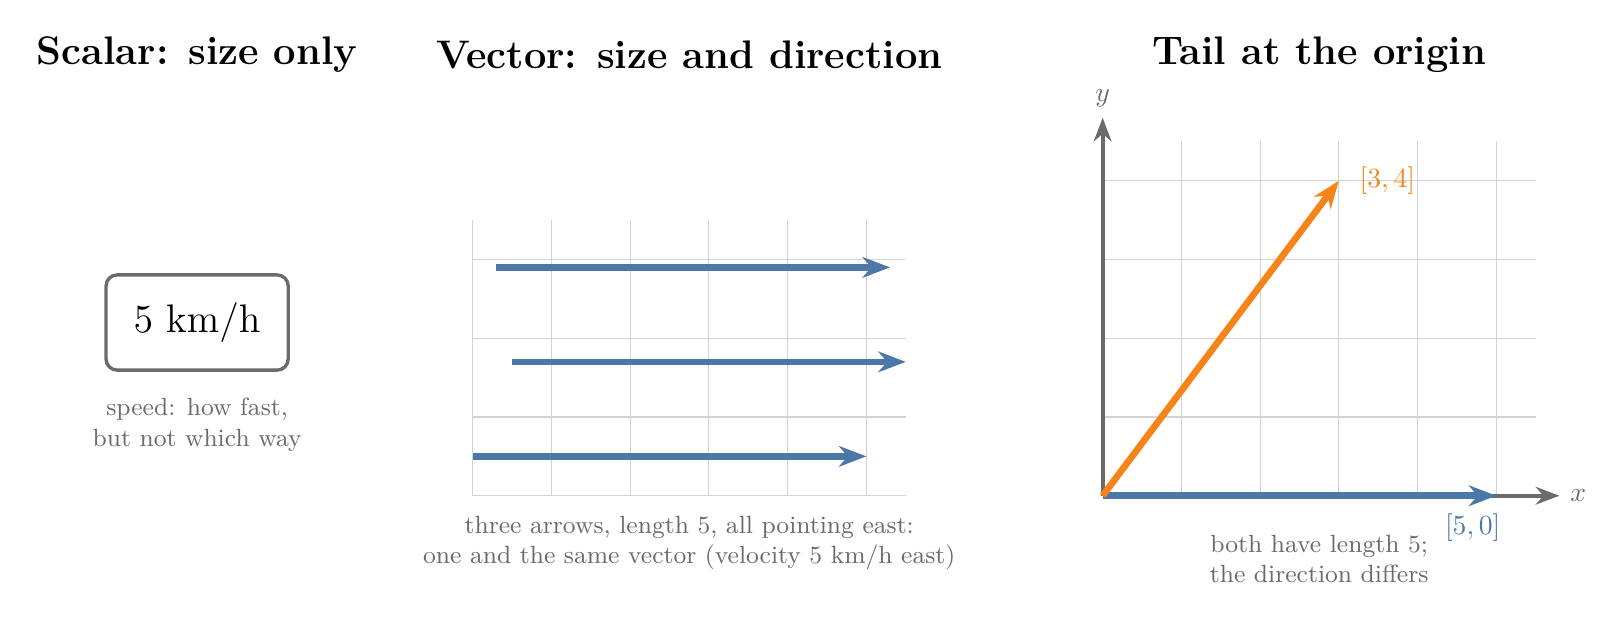
\begin{tikzpicture}
  % panel 1: scalar
  \node[title] at (1.5,5.6) {Scalar: size only};
  \node[draw=cgrey, rounded corners=4pt, inner sep=10pt, font=\Large] at (1.5,2.2) {5 km/h};
  \node[note] at (1.5,0.9) {speed: how fast,\\ but not which way};
  % panel 2: same vector, three places
  \begin{scope}[xshift=5cm]
    \node[title] at (2.75,5.6) {Vector: size and direction};
    \draw[cgrey!30, line width=0.4pt] (0,0) grid (5.5,3.5);
    \foreach \y/\x in {0.5/0, 1.7/0.5, 2.9/0.3} {
      \draw[-{Stealth[length=3.5mm]}, cblue, line width=2.4pt] (\x,\y) -- (\x+5,\y);
    }
    \node[note] at (2.75,-0.6) {three arrows, length 5, all pointing east:\\ one and the same vector (velocity 5 km/h east)};
  \end{scope}
  % panel 3: rooted at origin
  \begin{scope}[xshift=13cm]
    \node[title] at (2.75,5.6) {Tail at the origin};
    \draw[cgrey!30, line width=0.4pt] (0,0) grid (5.5,4.5);
    \draw[arrow, cgrey] (0,0) -- (5.8,0) node[right] {$x$};
    \draw[arrow, cgrey] (0,0) -- (0,4.8) node[above] {$y$};
    \draw[-{Stealth[length=3.5mm]}, cblue, line width=2.4pt] (0,0) -- (5,0) node[below left=2pt and -6pt, font=\bfseries] {$[5, 0]$};
    \draw[-{Stealth[length=3.5mm]}, corange, line width=2.4pt] (0,0) -- (3,4) node[right=3pt, font=\bfseries] {$[3, 4]$};
    \node[note] at (2.75,-0.8) {both have length 5;\\ the direction differs};
  \end{scope}
\end{tikzpicture}
\end{document}
